\chapter[Metodologia]{Metodologia}

Nesse capítulo são apresentadas e detalhadas as operações realizadas no processo de modelagem nos dois estudos de caso: a presença de corpos cetônicos no hálito e o respirador VESTA. Assim, inicialmente foi necessário realizar uma pesquisa para verificar e analisar as informações disponibilizadas na literatura recente, de forma a responder às principais questões de investigação deste trabalho: Qual a diferença de forma qualitativa de compostos orgânicos voláteis (COV) de acetona no hálito de um paciente diabético para uma pessoa saudável? Qual a diferenciação da máscara N95 tradicional e da máscara VESTA no controle de dissipação pandêmica do vírus SARS-CoV-2?

A partir do entendimento da fisiologia das áreas de estudo são implementadas hipóteses simplificadoras para facilitar a montagem do modelo análogo. Posteriormente, as variáveis ventilatórias e circulatórias, como: volume, fluxo e pressão são relacionadas aos componentes do domínio elétrico para a representação do modelo análogo. Dessa forma, essa analogia é empregada para entender o comportamento dinâmico do sistema respiratório e circulatório, seja em condições normais ou patológicas. Na sequência, aplicou-se a metodologia \textit{Bond Graph} (BG), inserindo o modelo final no software 20sim para encontrar as equações com a finalidade de obter a representação em espaços de estados do sistema.

Por conseguinte, para continuação do Trabalho de Conclusão de Curso tem-se a necessidade de realizar simplificações no modelo análogo, simulações no software \textit{Matlab} no domínio do tempo, da frequência, transitório e estacionário. Além do mais, deve-se determinar a estabilidade do sistema com a finalidade de regulamentar o comportamento do sistema a partir de variações de valores dos componentes eletrônicos, que determinam as características fisiológicas do grupo de pesquisa.    

\section{Descrição dos Sistemas}
\subsection{Bioengenharia da respiração}
\subsubsection{Corpos cetônicos na respiração}
O fígado recebe o suprimento sanguíneo de duas fontes: a artéria hepática e a veia porta. Sendo cerca de um terço do suprimento sanguíneo o sangue oxigenado da artéria hepática. Consequentemente, os outros dois terços do abastecimento é o sangue desoxigenado da veia porta do fígado \cite{Leungchavaphongse}, recebido dos capilares dos órgãos do sistema digestório e do baço, sangue esse que após uma refeição está rico em nutrientes absorvidos na digestão que posteriormente serão utilizados imediatamente ou armazenados  como fonte de energia a partir dos ácidos graxos ou da conversão do glicogênio em glicose. 

Sendo assim, após uma refeição, o nível da glicose sanguínea aumenta e estimula a produção de insulina nas ilhotas pancreáticas. Dessa forma, a ação do hormônio insulina tem como consequência o aumento do transporte da glicose sanguínea para as células do corpo por meio da difusão facilitada. Contudo, em casos de pacientes diabéticos, em que tem-se a baixa ou a inexistência produção de insulina, o que impossibilita o transporte de glicose para as células, dessa forma é necessária outra fonte de energia, assim, os ácidos graxos (grupo carboxila e em uma cadeia de hidrocarboneto) do tecido adiposo são metabolizados para a produção de energia por meio do trifosfato de adenosina (ATP), já que existe a impossibilidade do acesso das células à glicose \cite{Tortora}. 

O uso dos ácidos graxos ocorre em pacientes diabéticos quando há hiperglicemia, nome dado para altas taxas de glicose na corrente sanguínea. Entretanto, em indivíduos saudáveis a utilização dos ácidos graxos ocorre quando tem-se a necessidade da conservação das taxas de glicose sanguínea \cite{Tortora}. Posteriormente, é desencadeado o processo de lipólise \cite{Stanfield2014}, que é a separação do triglicerídeo em glicerol e ácidos graxos, e assim, os ácidos graxos são liberados para a corrente sanguínea com a finalidade de se tornarem a fonte para produção de ATP, a partir da $beta$-oxidação. Por conseguinte, no fígado é produzido o Acetil-CoA (acetilcoenzima A), que pode ser usado tanto para a gliconeogênese, processo para produção de ATP, quanto para a cetogênese, onde ocorre a produção da cetonas.

 Nas células do fígado no processo da cetogênese, o acetil-CoA acaba passando por um processo de conversão, gerando o ácido acetoacético, corpo cetônico primário instável. Sendo assim, uma parte do ácido acetoacético sofre fácil descarboxilação e se decompõe facilmente em acetona e CO2 \cite{Wang2013} e  também sofre uma degradação enzimática formando o ácido $\beta$-hidroxibutirato. Dessa forma, essas três substâncias são conhecidas como corpos cetônicos.
 
Em um organismo saudável assim que os ácidos graxos são metabolizados e os corpos cetônicos provenientes da reação no fígado entram na corrente sanguínea, os demais tecidos os utilizam imediatamente como fonte de energia e dessa forma, tem-se uma diminuição no nível de corpos cetônicos no corpo. Entretanto, existem períodos de $\beta$-oxidação excessiva, em que a produção de corpos cetônicos excede sua captação e uso pelas células. Sendo  esses períodos provenientes da realização de uma refeição rica em triglicerídeos; de períodos de jejum ou também hipoglicemia, já que poucos carboidratos estão disponíveis para o catabolismo e de situações de diabetes mellitus descontrolado ou não tratado, uma vez que, existe a falta ou a inexistência da produção de insulina, o que ocasiona a hiperglicemia e consequentemente entra uma quantidade inadequada de glicose nas células, dessa forma, os triglicerídios são necessários para a produção de ATP, o qual em consequência acelera o ritmo da lipólise.


\begin{figure}[H]
 \begin{center}
  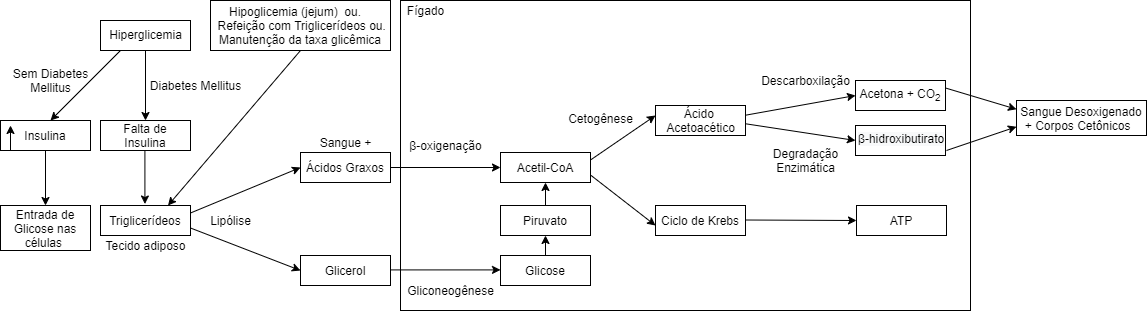
\includegraphics[width=\textwidth]{figuras/esq_figado.png}
  %\vspace{-15pt}
   \caption{{Esquemático da produção de acetona nas células do fígado}}\label{esq_figado}
  \end{center}
\end{figure}


Em seguida, o sangue desoxigenado do fígado com os corpos cetônicos, principalmente a acetona é drenado para as veias hepáticas. Entretanto, nestes três períodos em que ocorre a $\beta$-oxidação excessiva,  a qual ocasiona o aumento do nível de corpos cetônicos, que de maneira extrema ou prolongada pode levar à cetoacidose, um pH sanguíneo anormalmente baixo, já que os os corpos cetônicos são ácidos. Dessa forma, as veias hepáticas escoam na veia cava inferior o sangue desoxigenado e com acetona, até chegar no coração, pelo átrio direito e assim passa pela válvula tricúspide para chegar até o ventrículo direito. 

Posteriormente, a circulação pulmonar leva sangue desoxigenado e acetona do ventrículo direito para os alvéolos nos pulmões. Dessa forma, como a acetona é uma molécula pequena ela participa dos processos de difusão passiva na membrana respiratória, e o processo ocorre da área em que pressão parcial é maior para a área em que a pressão parcial é menor, sendo possível realizar a troca de O2 e CO2. A partir deste processo, o ar com CO2 e cetona é difundido para as vias aéreas (brônquios, traqueia, laringe e faringe) e posteriormente atinge-se a boca, e assim se torna presente no hálito. Portanto, a acetona no hálito passou a ser considerada um biomarcador para monitorar o estado cetótico de pessoas em jejum e pacientes diabéticos \cite{King2011}.

\begin{figure}[H]
 \begin{center}
  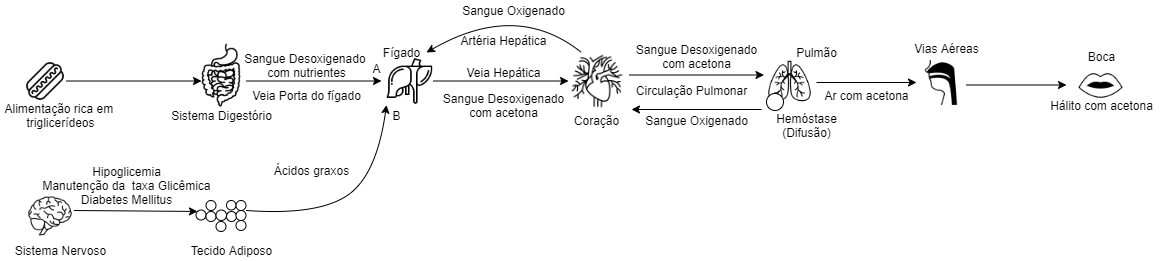
\includegraphics[width=\textwidth]{figuras/_esq_sist.png}
  %\vspace{-15pt}
   \caption{{Esquemático da presença da acetona no hálito A) após uma refeição rica em  triglicerídeos e B) pacientes em jejum ou diabéticos}}\label{esq_sistema}
  \end{center}
\end{figure}

\subsubsection{Vírus  SARS-CoV-2 na respiração}
\section{Hipóteses Simplificadoras}
\section{Modelos Análogos Eletrônicos}
\section{Representação Bond Graph}
\section{Matriz Espaço de Estados}

\newpage

\begin{landscape}
\begin{equation}\label{eq: estados_expandida0}
A
=  
\left[ \begin{matrix} 
\frac{-1}{R_{Vpi}C_{Vpi}}& 0 & 0 &\cdots  & 0\cr
0 & -\frac{Rs_{Vp}}{I_{Vp}} & -\left(Rs_{Vp1i}+\frac{1}{C_{Vp1i}}\right)&\cdots  & e_8\cr
0   & 0 & -\left(\frac{Rs_{Vp}}{I_{Vp}} + 1\right)\cdot\frac{1}{Rs_{Vp1i}}   & -\frac{1}{Rs_{Vp1i}C_{Vp1i}} &  \vdots   \cr
0 & 0 & -\left(\frac{Rs_{Vp}}{I_{Vp}} + 1\right)\cdot\frac{1}{Rs_{Vpf}}  & 0 & A_{(n,n)}\cr
\end{matrix} \right]
\end{equation}
\end{landscape}


\begin{equation}\label{eq: estados_expandida0}
B
=  
\left[ \begin{matrix} 
\frac{1}{R_{Vpi}} & 0 & \cdots  & B_{(1,i)}\cr
1 & B_{(2,2)} & \cdots  & B_{(2,i)}\cr
\frac{Se}{Rs_{Vp1i}}    & \vdots    & \ddots  & \vdots   \cr
B_{(n,1)} & B_{(n,2)} & \cdots  & B_{(n,i)}\cr
\end{matrix} \right] 
\end{equation}